% TODO Anhänge anfügen
% Wir haben dies jeweils über \chapter gelöst
% \includepdf[pages=-]{PDF-ANHANG}

\chapter{Aufgabenstellung}
\label{app:sec:Aufgabenstellung}

\includepdf[pages=-]{2020-02 Aufgabenstellung Movie Recommender}

\chapter{Sprintreviews}
\section*{Initiale Risikoanalyse}
Zu Beginn des Projektes wurden folgende Risiken erfasst:

\begin{figure}[htb]
	\centering
	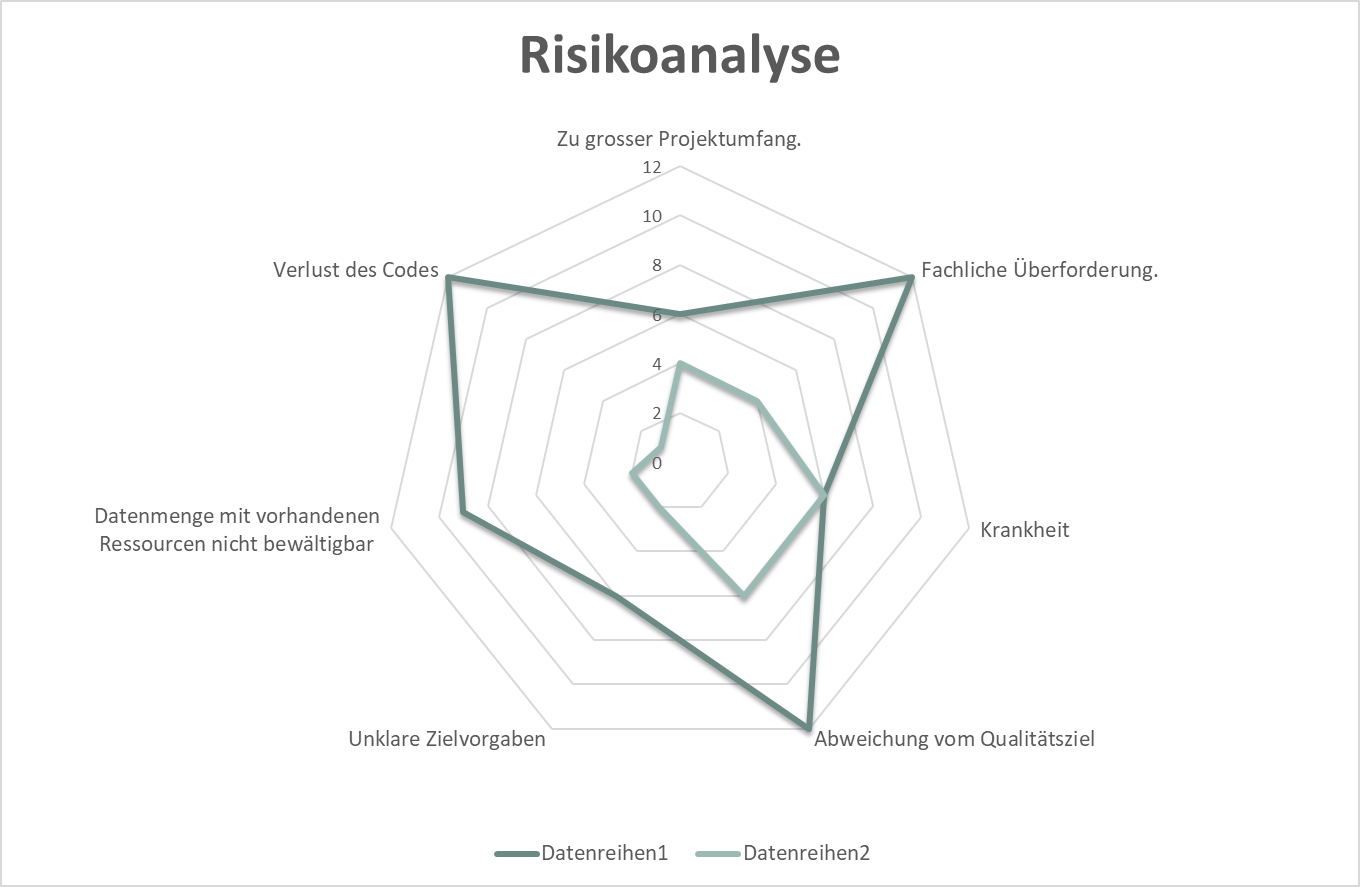
\includegraphics[keepaspectratio,width=\linewidth]{img/Initiale Risikoanalyse.png}
	\caption{Risikoanalyse}
	\label{fig:InitialeRisikoanalyse}
\end{figure}

\section*{Sprint 1 Review und Sprint 2 Planning}
Nach dem ersten Sprint wurden die Risiken wie folgt angepasst:
\begin{figure}[htb]
	\centering
	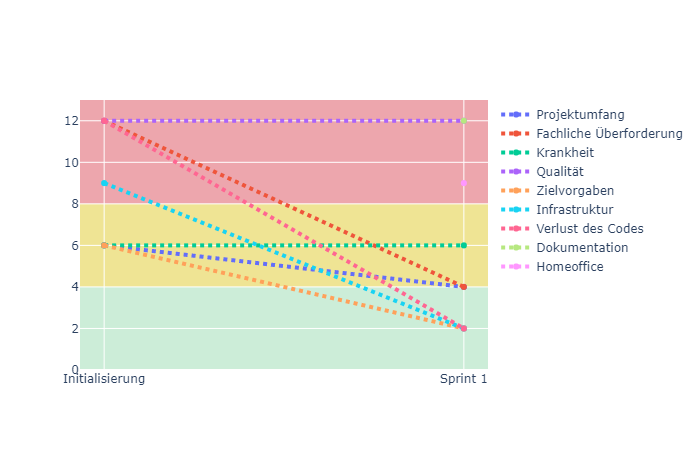
\includegraphics[keepaspectratio,width=\linewidth]{img/Risiken Sprint1.png}
	\caption{Risiken nach Sprint 1}
	\label{fig:Sprint 1 Risiken}
\end{figure}
Des weiteren wurde Sprint 2 geplant. 
\begin{figure}[htb]
	\centering
	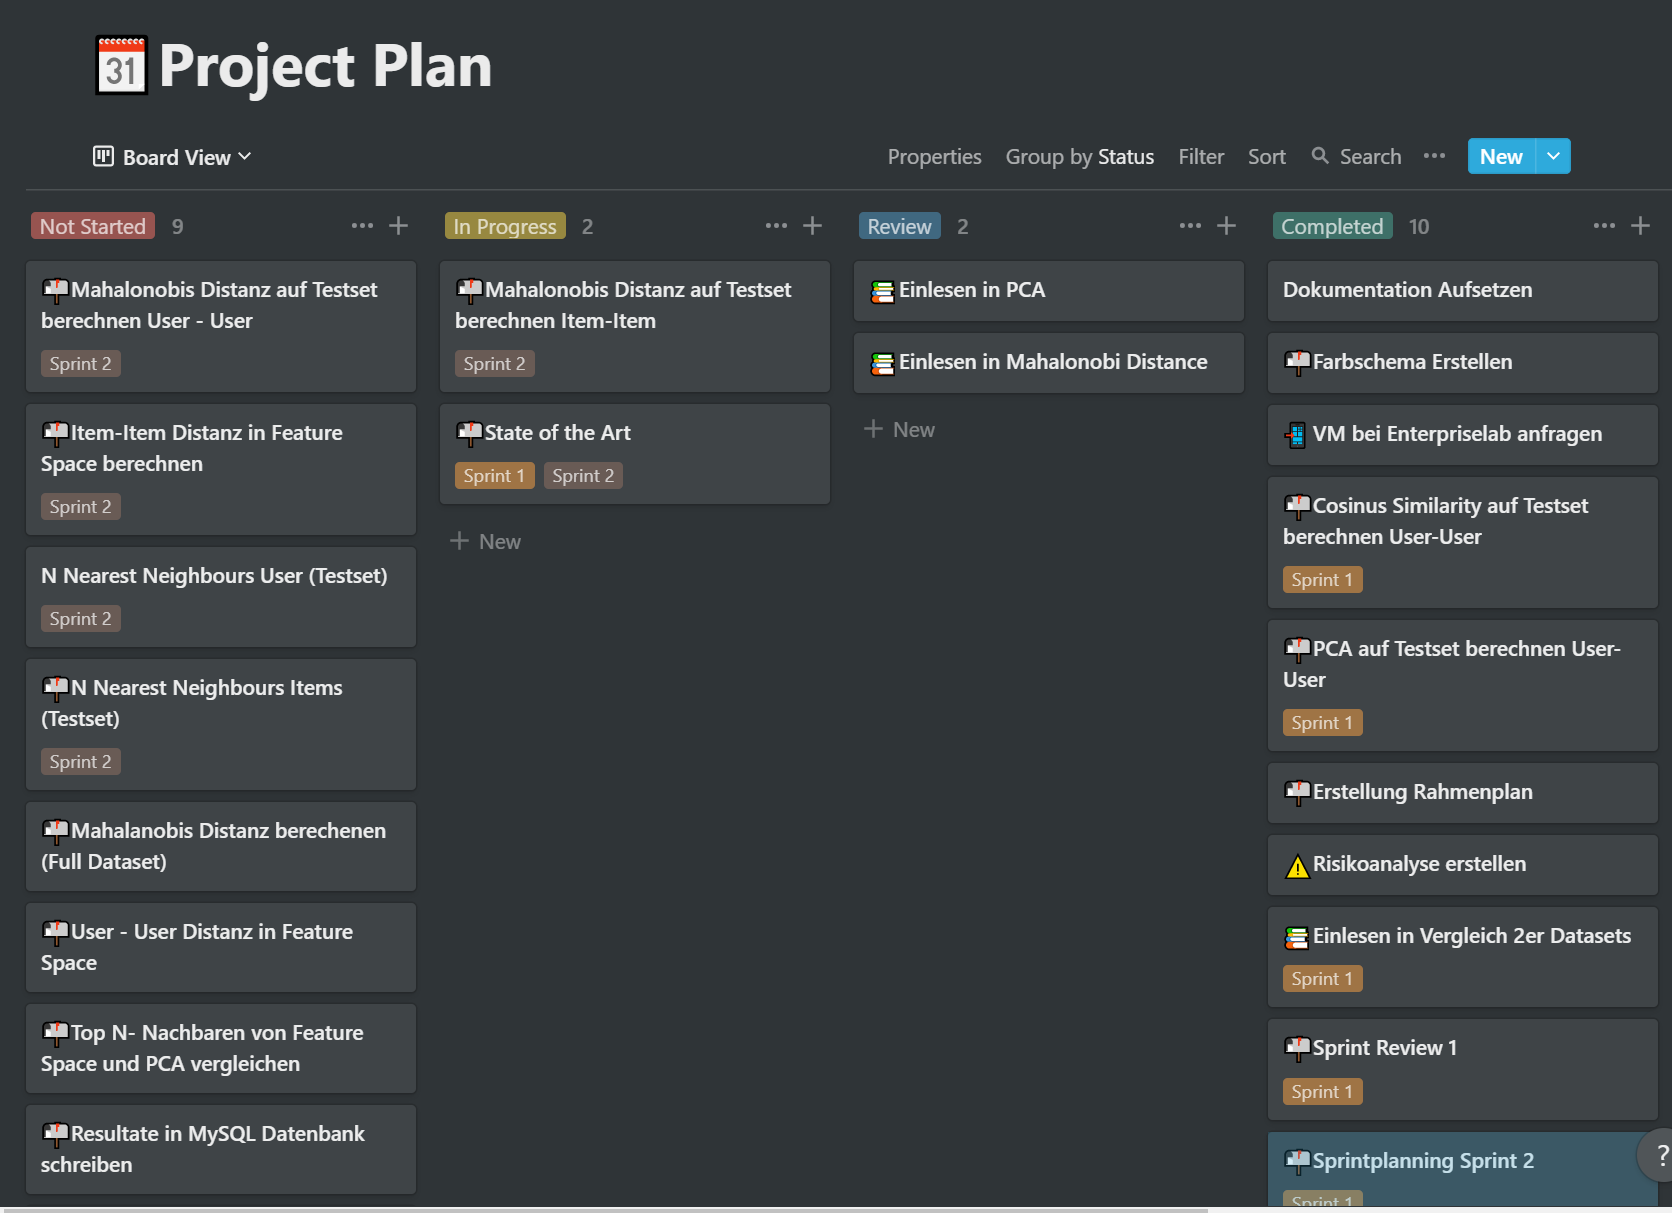
\includegraphics[keepaspectratio,width=\linewidth]{img/Projektboard Review Sprint1 Planning Sprint2.png}
	\caption{Projektboard Sprint 1 Review und Sprint 2 Planning}
	\label{fig:Sprint 1 Review}
\end{figure}

\section*{Sprint 2 Review und Sprint 3 Planning}
Nach dem zweiten Sprint wurden die Risiken wie folgt angepasst:
\begin{figure}[htb]
	\centering
	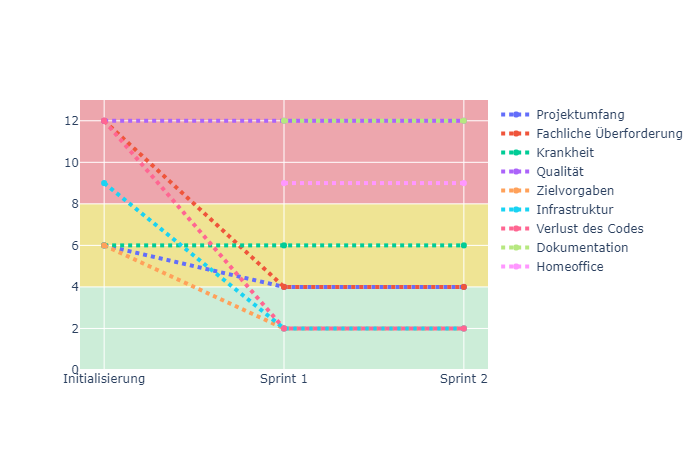
\includegraphics[keepaspectratio,width=\linewidth]{img/Risiken per Sprint Sprint2.png}
	\caption{Risiken nach Sprint 2}
	\label{fig:Sprint 2 Risiken}
\end{figure}
Des weiteren wurde Sprint 3 geplant. 
\begin{figure}[htb]
	\centering
	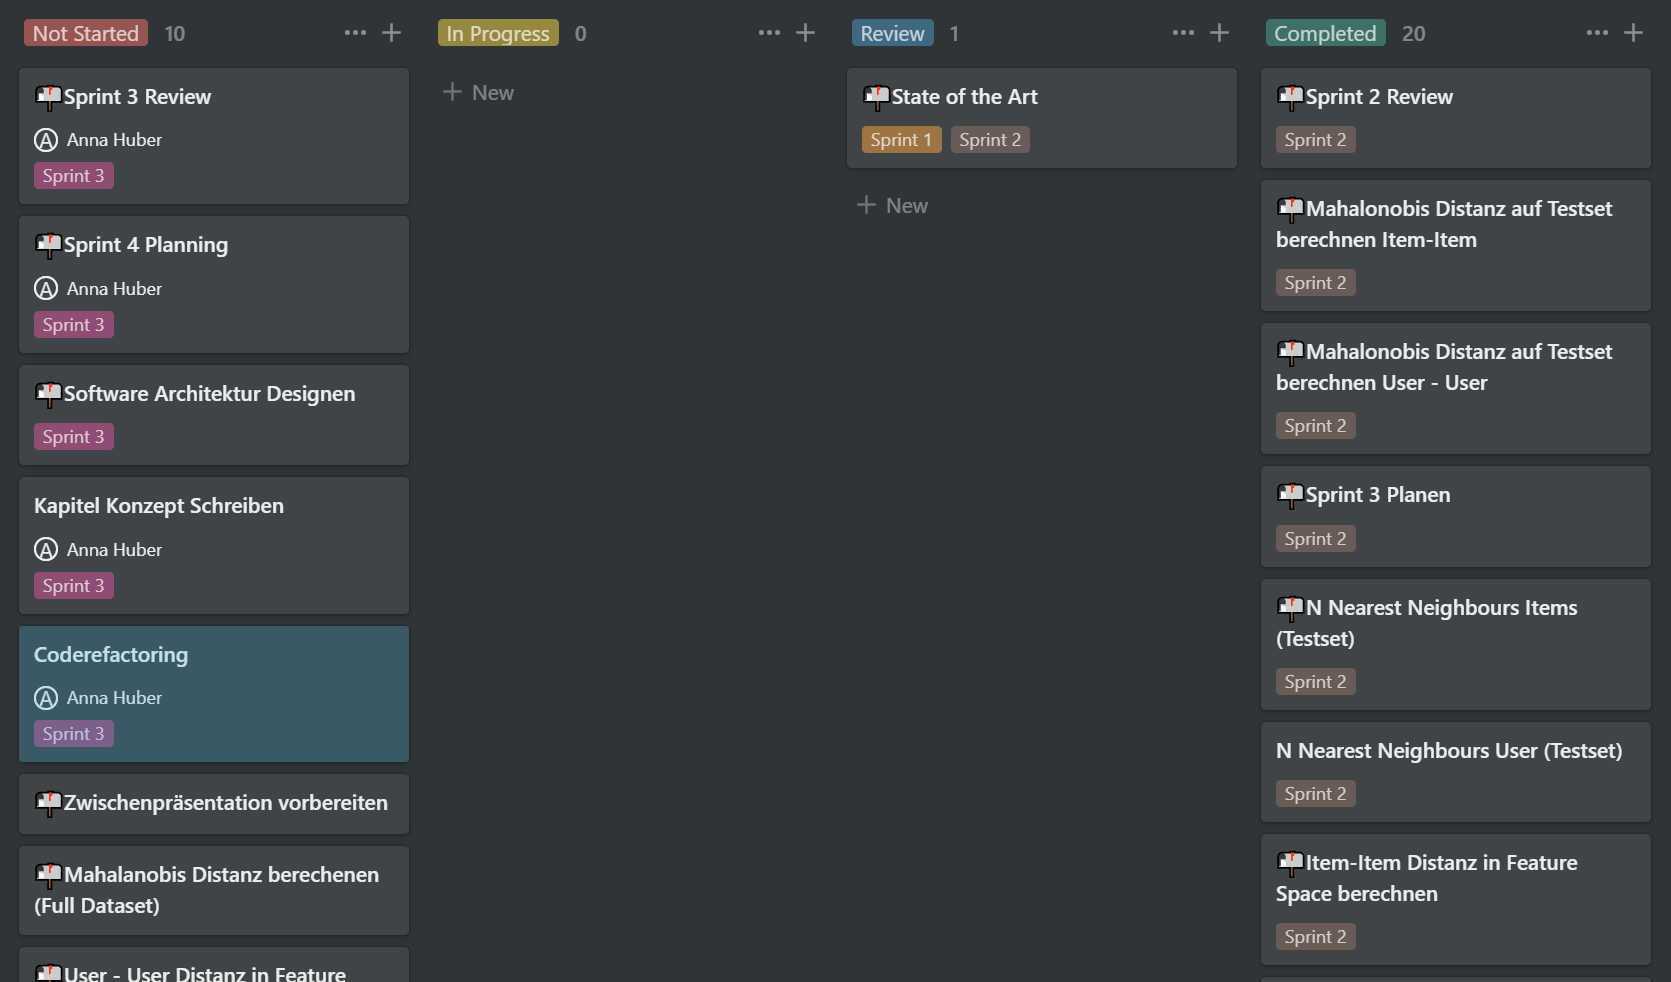
\includegraphics[keepaspectratio,width=\linewidth]{img/Projektboard Sprint Review 2.png}
	\caption{Projektboard Sprint 2 Review und Sprint 3 Planning}
	\label{fig:Sprint 2 Review}
\end{figure}
